\documentclass[tikz]{standalone}
\usepackage{pgfplots}

\pgfplotsset{compat=newest}
\pgfplotsset{
    yticklabel style={
        /pgf/number format/fixed,
        /pgf/number format/precision=2
    },
    scaled y ticks=false
}

\begin{document}
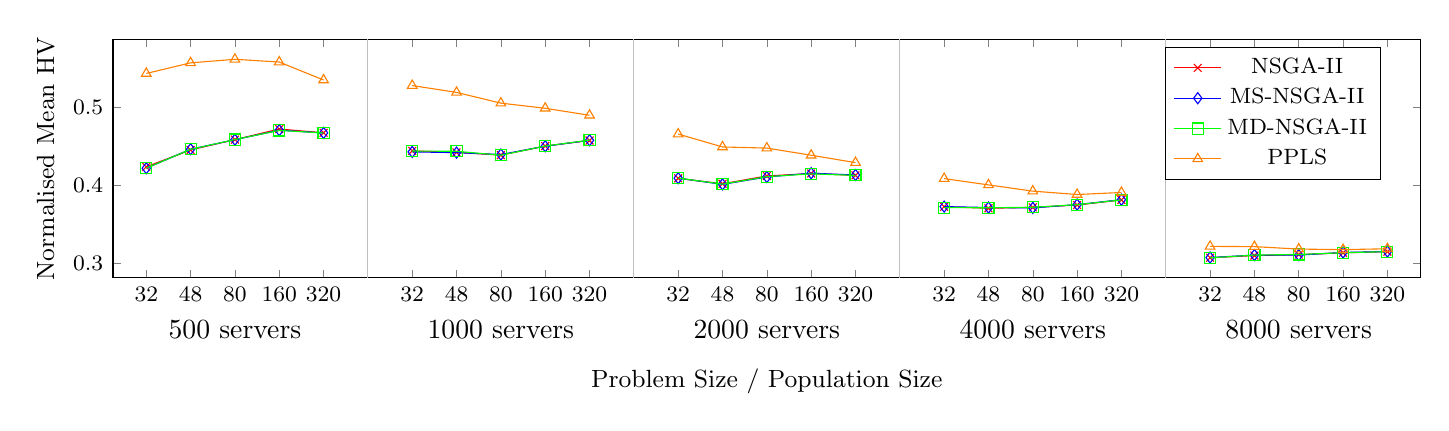
\begin{tikzpicture}

    \begin{axis}[
        footnotesize,
        max space between ticks=20pt,
        width=1.5\textwidth,
        height=0.38\textwidth,
        try min ticks=5,
        xtick=data,
        xticklabels={32, 48, 80, 160, 320, 32, 48, 80, 160, 320, 32, 48, 80, 160, 320, 32, 48, 80, 160, 320, 32, 48, 80, 160, 320},
        extra x ticks={5,11,17,23},
        extra x tick labels={},
        extra x tick style={
            grid=major,
            major tick length=0pt,
        },
        xlabel={Problem Size / Population Size},
        ylabel={Normalised Mean HV},
        xlabel style={
            yshift=-4ex,
        },
        enlarge x limits={abs=0.75},
        legend pos=north east,
        legend entries={
            {NSGA-II},
            {MS-NSGA-II},
            {MD-NSGA-II},
            {PPLS},
        },
        clip mode=individual,
    ]

    \addplot[
        mark=x,
        color=red
    ] table[
        x expr=\coordindex,
        y=PS
    ]{
        HV PS
        32 0.42394
        48 0.44562
        80 0.45884
        160 0.47243
        320 0.46763
        {} {}
        
        32 0.44438
        48 0.44246
        80 0.43893
        160 0.45064
        320 0.4577
        {} {}
        
        32 0.40914
        48 0.40215
        80 0.41222
        160 0.41531
        320 0.41303
        {} {}
        
        32 0.37269
        48 0.37073
        80 0.37189
        160 0.37489
        320 0.38145
        {} {}
        
        32 0.30723
        48 0.30997
        80 0.31123
        160 0.3135
        320 0.31506
        {} {}        
    };

    \addplot[
        mark=diamond,
        color=blue
    ] table[
        x expr=\coordindex,
        y=PS
    ]{
        HV PS
        32 0.42213
        48 0.44653
        80 0.45877
        160 0.47095
        320 0.46743
        {} {}
        
        32 0.4431
        48 0.44217
        80 0.43971
        160 0.45038
        320 0.45796
        {} {}
        
        32 0.40935
        48 0.40143
        80 0.41084
        160 0.41576
        320 0.41344
        {} {}
        
        32 0.37285
        48 0.37169
        80 0.37119
        160 0.37543
        320 0.38174
        {} {}
        
        32 0.3075
        48 0.31065
        80 0.3106
        160 0.31401
        320 0.31514
        {} {}          
    };

    \addplot[
        mark=square,
        color=green
    ] table[
        x expr=\coordindex,
        y=PS
    ]{
        HV PS
        32 0.42225
        48 0.44636
        80 0.45894
        160 0.47064
        320 0.46741
        {} {}
        
        32 0.4442
        48 0.44384
        80 0.43887
        160 0.4506
        320 0.45816
        {} {}
        
        32 0.40945
        48 0.40169
        80 0.41131
        160 0.41489
        320 0.41292
        {} {}
        
        32 0.37152
        48 0.37143
        80 0.37197
        160 0.37533
        320 0.38148
        {} {}
        
        32 0.30705
        48 0.31063
        80 0.31141
        160 0.31364
        320 0.31506
        {} {}                      
    };

    \addplot[
        mark=triangle,
        color=orange
    ] table[
        x expr=\coordindex,
        y=PS
    ]{
        HV PS
        32 0.54377
        48 0.55742
        80 0.56196
        160 0.55844
        320 0.53537
        {} {}
        
        32 0.52827
        48 0.51946
        80 0.50569
        160 0.49909
        320 0.4901
        {} {}
        
        32 0.46596
        48 0.44944
        80 0.44799
        160 0.4388
        320 0.4293
        {} {}
        
        32 0.40881
        48 0.40074
        80 0.39272
        160 0.38837
        320 0.391
        {} {}
        
        32 0.3218
        48 0.32146
        80 0.31835
        160 0.31762
        320 0.31876
        {} {}         
    };

    \begin{scope}[
        every label/.append style={
            label distance=2ex,
        },
    ]
        \node [label=below:500 servers]
            at (axis cs:2,\pgfkeysvalueof{/pgfplots/ymin}) {};
        \node [label=below:1000 servers]
            at (axis cs:8,\pgfkeysvalueof{/pgfplots/ymin}) {};
        \node [label=below:2000 servers]
            at (axis cs:14,\pgfkeysvalueof{/pgfplots/ymin}) {};
        \node [label=below:4000 servers]
            at (axis cs:20,\pgfkeysvalueof{/pgfplots/ymin}) {};
        \node [label=below:8000 servers]
            at (axis cs:26,\pgfkeysvalueof{/pgfplots/ymin}) {};
    \end{scope}
    \end{axis}
\end{tikzpicture}
\end{document}